\documentclass[runningheads]{llncs}
\usepackage{graphicx}
\usepackage{booktabs}
\usepackage{amsmath}
\usepackage{float}
\usepackage{tabularx}
\usepackage{enumitem}
\setlist{itemsep=2pt,topsep=4pt,parsep=0pt,partopsep=0pt}

% Force each \section to start on a new page
\let\oldsection\section
\renewcommand{\section}{\clearpage\oldsection}

\title{EALAI: An Explainable and Auditable Legal AI Framework\\
with Empirical Evaluation on Singapore Statutory Law}
\titlerunning{EALAI: Explainable and Auditable Legal AI}

\author{Mohammed Iqbal Khan\inst{1}}
\institute{Department of Data Science and Engineering,\\
Manipal University Jaipur, India\\
\email{sheranidanish12@gmail.com}}

\begin{document}
\maketitle

\begin{abstract}
Legal AI chatbots built on large language models frequently hallucinate statutory
references and provide no way to trace how an answer was produced. This paper presents
EALAI, a legal advisory system that combines hybrid retrieval-augmented generation
with a 20-rule symbolic consistency engine and SHA-256 tamper-evident audit logging.
The system retrieves from a corpus of 48 Singapore statutory PDFs using Reciprocal
Rank Fusion over BM25 and dense retrieval, then cross-checks every LLM response
against domain-specific legal rules before logging the full interaction.

We evaluate EALAI on a 200-question benchmark across three experiments. Dense
retrieval reduces hallucination from 42\% (no-retrieval baseline) to 20\% and
improves citation accuracy from 0.580 to 0.800. Hybrid retrieval achieves the best
raw recall (Hit@5 = 72.5\%) but unexpectedly underperforms on end-to-end citation
accuracy (0.645), suggesting that context coherence matters more than breadth for LLM
attribution. A refusal calibration sweep over ten thresholds identifies $\theta=0.45$
as the optimal operating point with 3\% false positives.

\keywords{Legal AI \and Retrieval-Augmented Generation \and Explainable AI \and
Symbolic Reasoning \and Audit Trails \and Singapore Law}
\end{abstract}

%---------------------------------------------------------------------
\section{Introduction}
%---------------------------------------------------------------------

AI-powered legal chatbots are increasingly used for document review, compliance
checks, and basic legal guidance~\cite{b2,b4}. The core risk is that language models
generate plausible but inaccurate text. When a system cites the wrong statute or
invents a section number, the person relying on that advice may face real
consequences~\cite{b1,b8}. Tools like DoNotPay have demonstrated both the potential
and the limitations of automated legal assistance~\cite{b3}.

Three failure modes recur in existing systems: (1) hallucination of statutory content,
(2) absence of citation provenance, and (3) unauditable reasoning incompatible with
emerging governance requirements such as the EU AI Act~\cite{b6} and digital ethics
frameworks~\cite{b5}. Most production systems treat explainability as an afterthought
rather than an architectural requirement~\cite{b7}.

This paper presents EALAI, a working system that addresses all three failure modes.
Our contributions are:

\begin{enumerate}
  \item A hybrid RAG pipeline combining BM25~\cite{b11} and dense retrieval via
        Reciprocal Rank Fusion~\cite{b12}, with a 20-rule symbolic consistency engine
        that cross-checks LLM output against known Singapore legal rules.
  \item A SHA-256 tamper-evident audit logger that records every interaction with
        deterministic hashing for post-hoc verification.
  \item Empirical evaluation on a 200-question benchmark showing that RAG reduces
        hallucination by 22 percentage points, along with the finding that retrieval
        coverage and end-to-end citation accuracy are not positively correlated.
\end{enumerate}

%---------------------------------------------------------------------
\section{Related Work}
%---------------------------------------------------------------------

\textbf{Rule-based legal AI.}
Early systems such as Taxman~\cite{b9} encoded legal reasoning as IF-THEN
chains. These produced auditable reasoning but could not scale beyond narrow
domains.

\textbf{Neural approaches.}
Transformer models (BERT through GPT-4) enabled broad legal NLP without explicit
rules. Domain-specific efforts include DISC-LawLLM~\cite{b14} for Chinese legal
services and the Indian Legal Documents Corpus~\cite{b15} for court judgment
prediction. Commercial products such as Harvey AI and CoCounsel have reached
production, but hallucinated citations and opaque reasoning remain
persistent problems~\cite{b1,b8}.

\textbf{Retrieval-augmented generation.}
RAG~\cite{b10} reduces hallucination by conditioning LLM output on retrieved
documents rather than parametric memory. Hybrid search combining dense and sparse
retrieval tends to outperform either method alone, and chunk-level metadata is
important for verifiable citations~\cite{b7}. Automated evaluation frameworks such as
RAGAS~\cite{b13} have been developed to assess RAG pipeline quality.

\textbf{Gap.}
No existing open-source legal AI system, to our knowledge, combines retrieval-based
grounding with symbolic consistency checking and cryptographic audit logging. EALAI
integrates all three as first-class architectural components.

%---------------------------------------------------------------------
\section{System Architecture}
%---------------------------------------------------------------------

Table~\ref{tab:arch} shows the eight-stage pipeline. Stages 1--6 form the RAG core;
stages 7--8 are the EALAI additions.

\begin{table}[H]
\centering
\caption{EALAI eight-stage pipeline from user input to audited response.}
\label{tab:arch}
\small
\begin{tabular}{clp{7.5cm}}
\toprule
\textbf{Stage} & \textbf{Module} & \textbf{Function} \\
\midrule
1 & Intent Classifier    & Keyword-based domain tagging (employment / contract / PDPA) \\
2 & Entity Extractor     & spaCy NER: persons, dates, organisations, locations \\
3 & KB Retriever         & BM25 + dense search fused via RRF ($k=60$), top-$k$ chunks \\
4 & Prompt Builder       & Jinja2 template: context, history, intent/entity slots \\
5 & LLM                  & \texttt{llama-3.1-8b-instant} via Groq ($T=0.1$) \\
6 & Response Formatter   & Regex section parser $\rightarrow$ structured dict \\
\midrule
7 & Symbolic Engine      & 20-rule \texttt{SingaporeLegalEngine}: consistency flag \\
8 & Audit + Citation     & SHA-256 JSONL logger; citation accuracy scorer \\
\bottomrule
\end{tabular}
\end{table}

\subsection{Retrieval Pipeline (Stages 1--3)}

\textbf{Preprocessing.} A keyword-based intent classifier identifies legal domains
(employment, contract, PDPA) and spaCy extracts named entities (locations, persons,
dates). Both outputs are injected into the prompt.

\textbf{Corpus.} 48 Singapore statutory PDFs are chunked using paragraph-boundary
splitting with token-aware sizing (target 500--1000 tokens, 15\% overlap) and indexed
in ChromaDB with \texttt{all-MiniLM-L6-v2} embeddings (384 dimensions).

\textbf{Retrieval modes.} The system supports three modes:
\begin{itemize}
  \item \textbf{BM25 Okapi}~\cite{b11} ($k_1=1.5$, $b=0.75$) for keyword retrieval.
  \item \textbf{Dense search} via cosine similarity over chunk embeddings.
  \item \textbf{Hybrid (default):} both run independently and are merged using
        Reciprocal Rank Fusion~\cite{b12} with $k=60$:
        $\text{score}(d) = \sum_i \frac{1}{k + \text{rank}_i(d)}$.
\end{itemize}

\subsection{Generation and Formatting (Stages 4--6)}

A Jinja2 template injects conversation history, retrieved chunks (with source
citations), intent/entity slots, and output format instructions into the prompt.
The LLM (\texttt{llama-3.1-8b-instant} via Groq, $T=0.1$) must respond in five
labelled sections: Applicable Law, Reasoning, Answer, Limitations, and Disclaimer,
plus a confidence tag. A response formatter parses these sections via regex-based
header detection.

\subsection{Symbolic Consistency Engine (Stage 7)}

The \texttt{SingaporeLegalEngine} holds 20 IF-THEN rules encoded as Python
dataclasses, covering the Employment Act 1968 (rules 1--8), Contract Law (9--12), and
PDPA (13--20). Each rule carries a trigger condition, statute name, and section
reference. The \texttt{check\_consistency()} function compares the matched statute
against the LLM's stated Applicable Law, producing a consistency flag
(\texttt{True}/\texttt{False}/\texttt{None}).

\subsection{Audit Logger and Citation Checker (Stage 8)}

Every interaction is appended to an audit log as a JSON object. A SHA-256 hash is
computed over all field values (sorted by key, pipe-joined) for tamper detection. A
citation checker extracts \texttt{[Act Name, Section X]} patterns from the LLM output
via regex and verifies each against retrieved chunk texts, producing a
\texttt{citation\_accuracy} score in $[0, 1]$.

%---------------------------------------------------------------------
\section{Evaluation}
%---------------------------------------------------------------------

\subsection{Benchmark}

We constructed a benchmark of 200 questions (74 employment, 62 contract, 64 PDPA)
with gold-standard answers, statute references, and chunk IDs. For the refusal
calibration experiment, 100 additional out-of-scope (OOS) queries were annotated
across 8 categories (wrong jurisdiction, non-legal, fictional case, etc.).

\subsection{Retrieval Quality}

Table~\ref{tab:retrieval} reports Precision@$k$ and Hit@$k$ for $k \in \{3, 5\}$
across 142 scoreable questions (58 excluded for non-statute gold references).

\begin{table}[H]
\centering
\caption{Retrieval benchmark ($n=142$).}
\label{tab:retrieval}
\begin{tabular}{lcccc}
\toprule
\textbf{Retriever} & \textbf{P@3} & \textbf{Hit@3} & \textbf{P@5} & \textbf{Hit@5} \\
\midrule
BM25   & 0.279 & 50.7\% & 0.249 & 56.3\% \\
Dense  & 0.289 & 57.8\% & 0.249 & 65.5\% \\
\textbf{Hybrid (RRF)} & \textbf{0.322} & \textbf{58.5\%} & \textbf{0.293} & \textbf{72.5\%} \\
\bottomrule
\end{tabular}
\end{table}

Hybrid retrieval consistently outperforms either retriever alone. The largest gap is
at Hit@5 (72.5\% vs.\ 65.5\% for dense), confirming that RRF fusion recovers relevant
chunks missed by individual retrievers.

\subsection{End-to-End Evaluation}

Four retrieval conditions were evaluated across all 200 questions. Following the
approach of automated RAG evaluation~\cite{b13}, each response was scored for
hallucination rate and citation accuracy (Table~\ref{tab:e2e},
Figure~\ref{fig:eval}).

\begin{table}[H]
\centering
\caption{End-to-end results across four retrieval conditions ($n=200$).}
\label{tab:e2e}
\begin{tabular}{lccc}
\toprule
\textbf{Retriever} & \textbf{Hallucination} & \textbf{Citation Acc.} & \textbf{Latency} \\
\midrule
None (baseline) & 42\%            & 0.580 & 30.7\,s \\
BM25            & 22\%            & 0.784 & 34.3\,s \\
\textbf{Dense}  & \textbf{20\%}   & \textbf{0.800} & 32.5\,s \\
Hybrid          & 36\%            & 0.645 & 33.1\,s \\
\bottomrule
\end{tabular}
\end{table}

\begin{figure}[t]
\centering
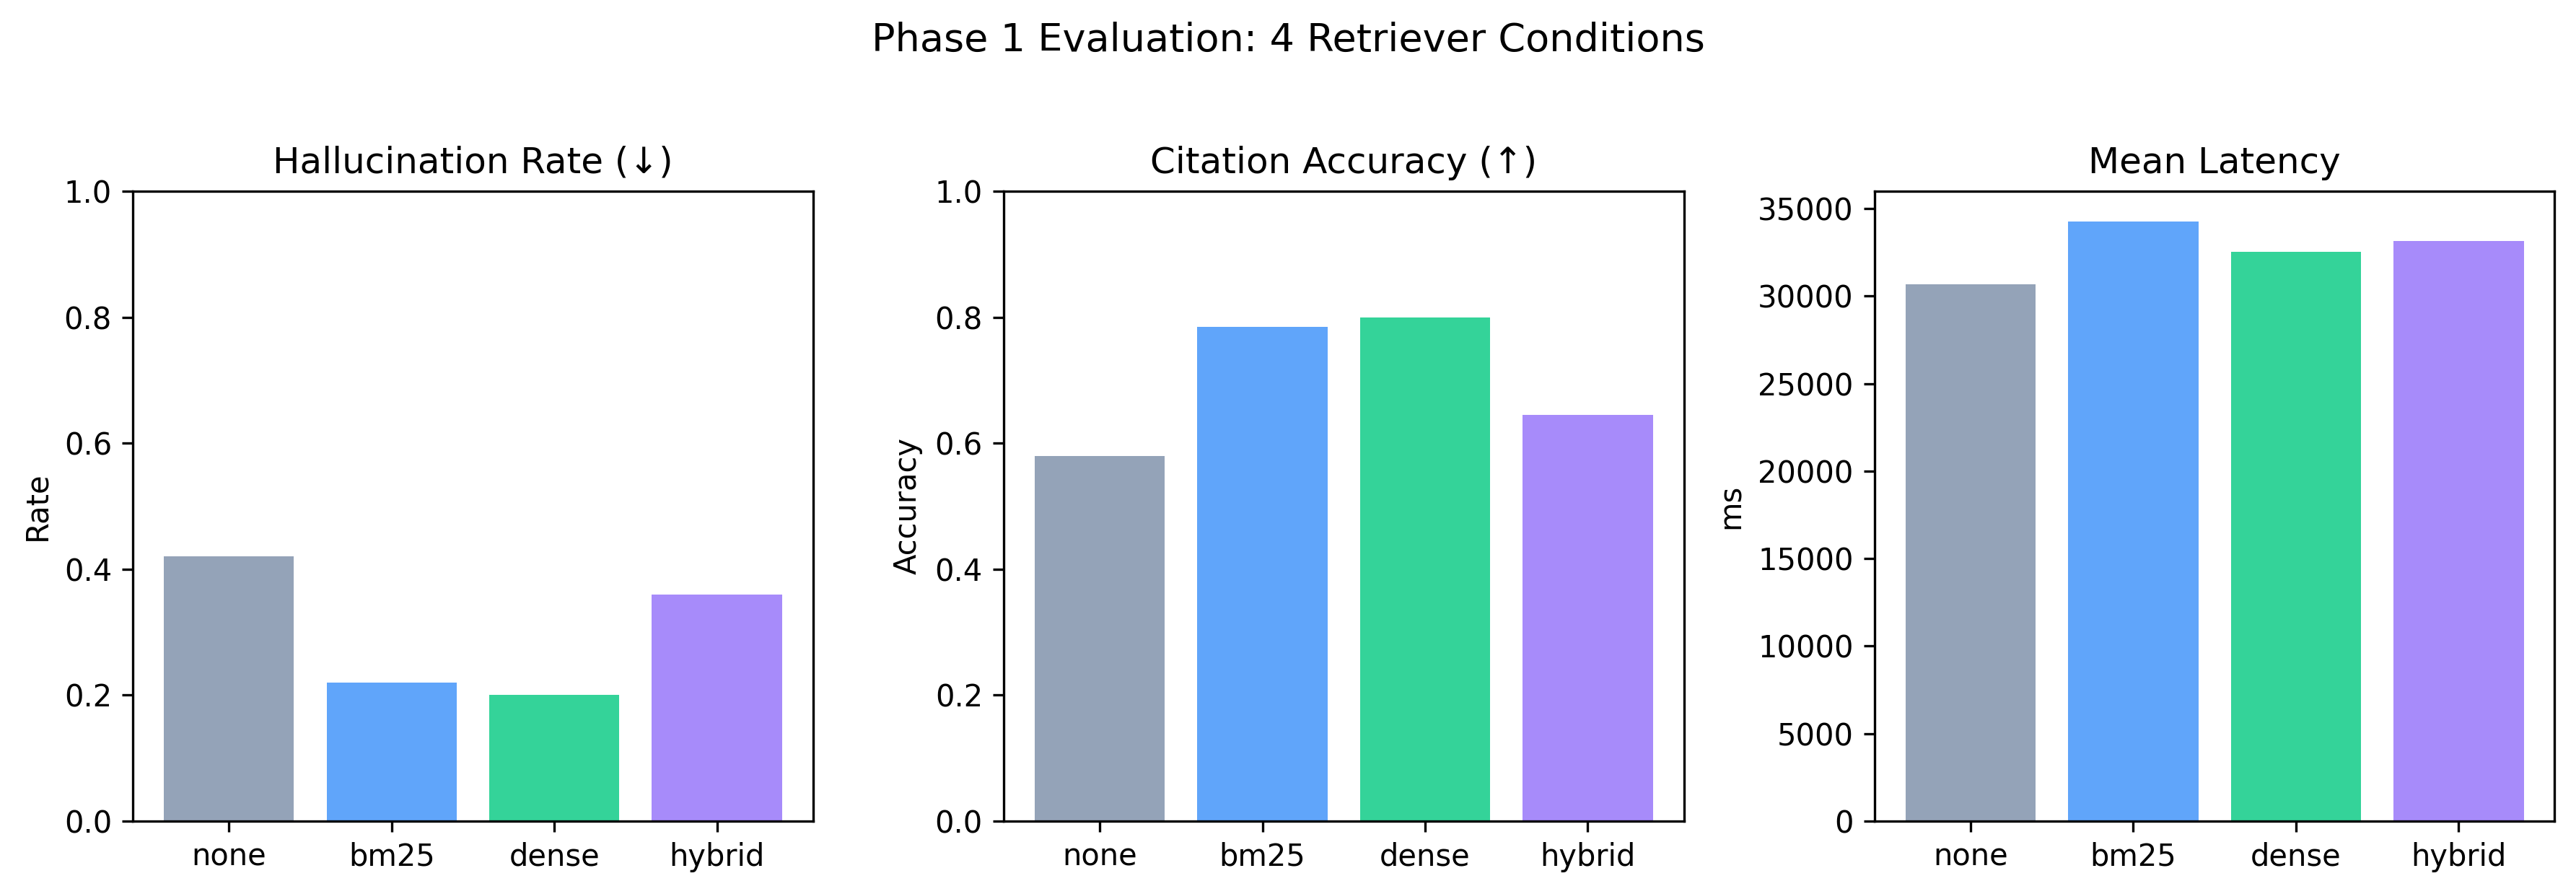
\includegraphics[width=\textwidth]{figures/fig2_evaluation_summary.png}
\caption{Hallucination rate, citation accuracy, and latency across four conditions.
Latency includes Groq API round-trip time.}
\label{fig:eval}
\end{figure}

Dense retrieval achieves the best end-to-end quality: 20\% hallucination rate and
0.800 citation accuracy. The key finding is that hybrid retrieval, despite winning on
raw retrieval recall (Table~\ref{tab:retrieval}), underperforms on citation accuracy
(0.645 vs.\ 0.800). The RRF-merged context introduces topical diversity that the LLM
cannot reliably attribute, producing a dissociation between retrieval coverage and
response quality.

\subsection{Refusal Calibration}

The refusal mechanism rejects queries where the maximum retrieval score falls below a
threshold $\theta$. We swept $\theta \in \{0.20, 0.25, \ldots, 0.70\}$ using 100 OOS
and 100 in-corpus queries per threshold (Figure~\ref{fig:refusal}).

\begin{figure}[t]
\centering
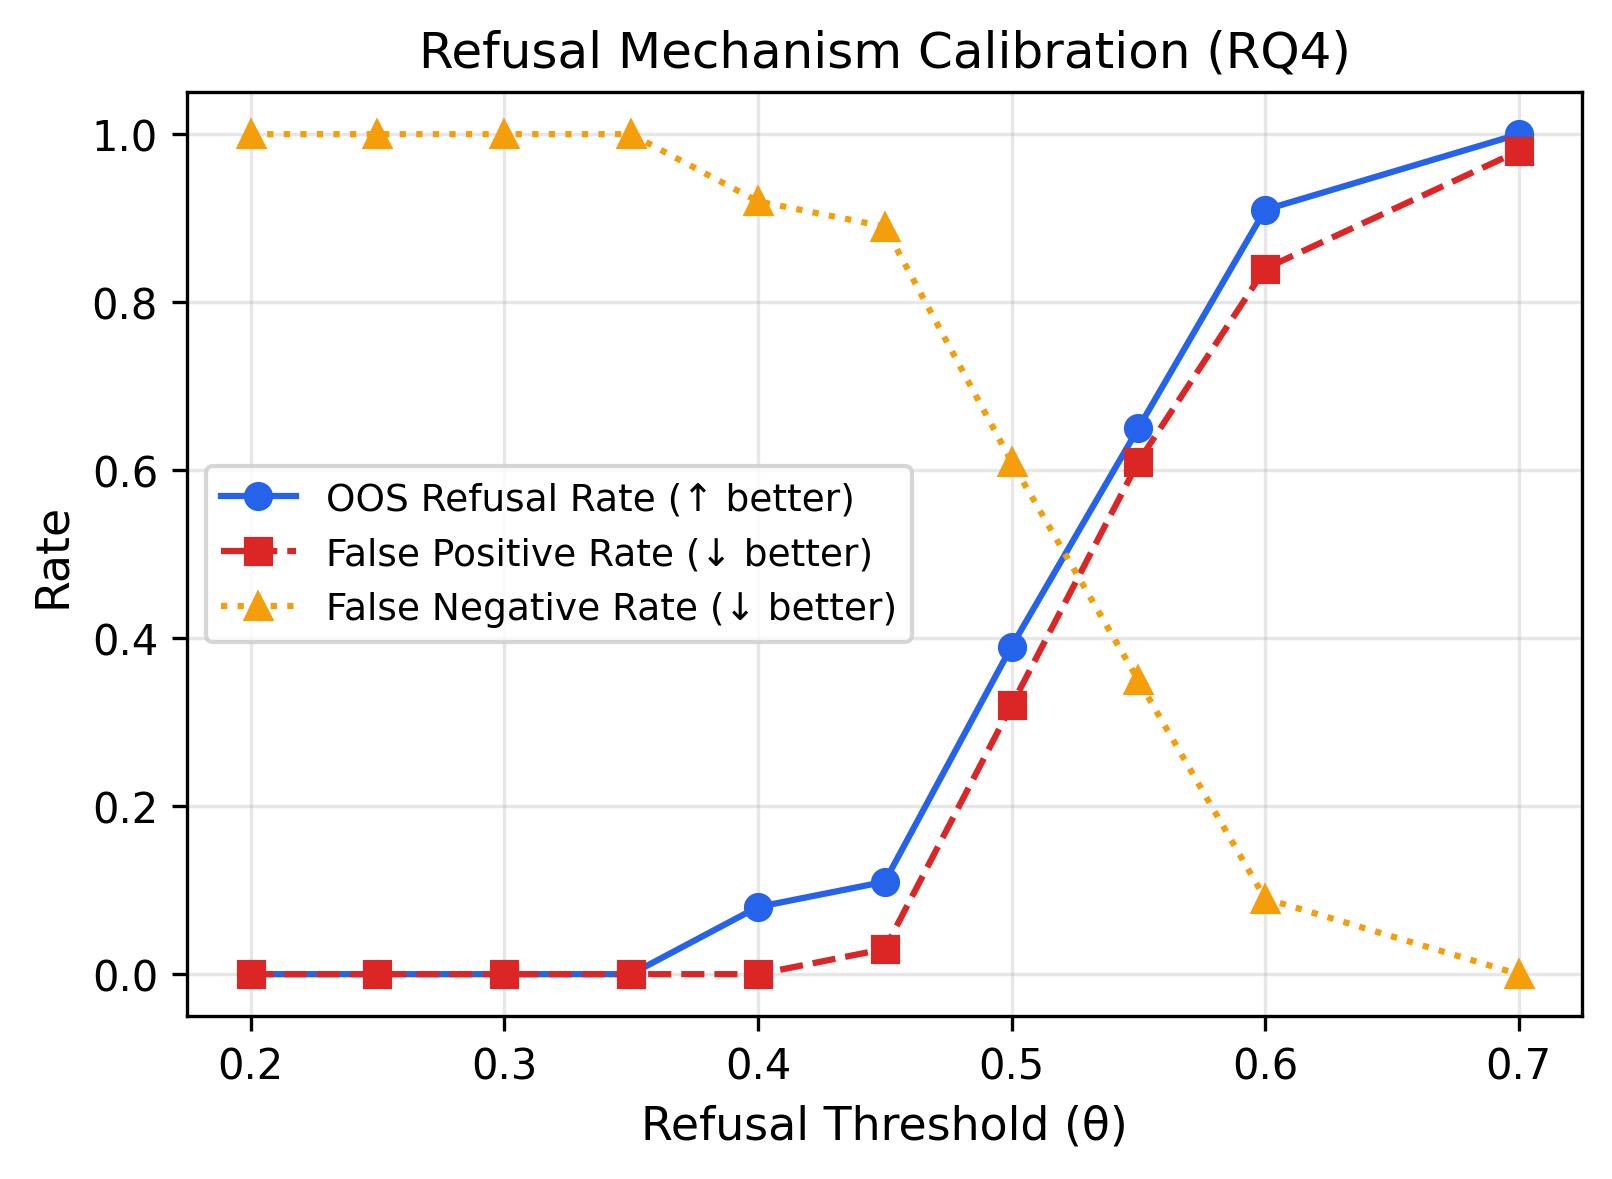
\includegraphics[width=0.78\textwidth]{figures/fig1_refusal_curve.png}
\caption{Refusal calibration sweep. The false positive rate jumps from 3\% to 32\%
between $\theta=0.45$ and $\theta=0.50$.}
\label{fig:refusal}
\end{figure}

The curve shows a sharp cliff between $\theta=0.45$ and $\theta=0.50$: the false
positive rate jumps from 3\% to 32\% for only a 28pp gain in OOS recall. The
recommended operating point is $\theta=0.45$.

%---------------------------------------------------------------------
\section{Discussion}
%---------------------------------------------------------------------

\subsection{Key Findings}

\textbf{RAG substantially reduces hallucination.} Dense retrieval cuts the
hallucination rate from 42\% to 20\%, a 22pp reduction, confirming that grounding LLM
output in verified statutory text is effective even with a small (8B parameter) model.

\textbf{Retrieval coverage $\neq$ response quality.} Hybrid retrieval achieves the
best Hit@5 (72.5\%) but the worst citation accuracy among RAG conditions (0.645).
This suggests that the LLM's ability to correctly attribute claims degrades when the
context contains topically diverse chunks from multiple retrieval signals. For
downstream citation quality, a focused, high-precision context appears preferable to a
broad, high-recall one.

\textbf{Refusal threshold has a sharp cliff.} The precision-recall tradeoff for the
refusal mechanism is non-linear, with a single 0.05 threshold step producing a
tenfold increase in false positives. This highlights the need for careful calibration
rather than relying on default values.

\subsection{Limitations}

\begin{itemize}
  \item \textbf{Automated evaluation only.} Citation accuracy is computed via regex
        matching, not expert annotation. Subtle hallucinations (correct statute, wrong
        interpretation) may be missed.
  \item \textbf{Small model.} All experiments use Llama-3.1-8b-instant. Results may
        not generalize to larger models that handle diverse contexts differently.
  \item \textbf{Corpus scope.} The 48-PDF corpus covers three domains within
        Singapore law. The system cannot assess its own blind spots within covered
        domains.
  \item \textbf{Rule coverage.} The 20-rule symbolic engine covers a subset of
        scenarios. Queries between rules receive no consistency check.
  \item \textbf{No user study.} Perceived explainability and response clarity have not
        been measured with human participants.
\end{itemize}

%---------------------------------------------------------------------
\section{Conclusion}
%---------------------------------------------------------------------

We presented EALAI, a legal AI system combining hybrid RAG retrieval, a 20-rule
symbolic consistency engine, and SHA-256 tamper-evident audit logging. Evaluation on a
200-question Singapore law benchmark shows that retrieval-augmented generation reduces
hallucination by 22 percentage points and that retrieval coverage does not
automatically translate into citation accuracy. The refusal calibration sweep
identifies a sharp precision cliff that underscores the importance of threshold
tuning.

Future work includes expanding the symbolic rule base, conducting a user study with
legal aid recipients, developing a composite Explainability Index metric, and
evaluating on larger language models and additional jurisdictions.

%---------------------------------------------------------------------
\begin{thebibliography}{15}

\bibitem{b1}
Ogunsan, A., Johnson, N.: The use of chatbots in providing free legal guidance:
benefits and limitations. J.\ Legal Technology (2025)

\bibitem{b2}
Susskind, R.: Tomorrow's Lawyers: An Introduction to Your Future, 2nd edn.
Oxford University Press (2017)

\bibitem{b3}
Hagan, M.: DoNotPay and beyond: how automated tools are democratizing access to
justice. J.\ Legal Innovation (2021)

\bibitem{b4}
Dale, R.: The return of the chatbots. Natural Language Engineering
\textbf{22}(5), 811--817 (2016)

\bibitem{b5}
Floridi, L.: Translating principles into practices of digital ethics.
Philosophy \& Technology \textbf{32}, 185--193 (2019)

\bibitem{b6}
European Commission: Proposal for a regulation laying down harmonised rules on
artificial intelligence (AI Act). Brussels (2021)

\bibitem{b7}
Karamcheti, K., et al.: LLMs in law: towards explainable and grounded legal
reasoning. arXiv:2406.04136 (2024)

\bibitem{b8}
Ogunsan, A., Johnson, N.: Limitations of legal chatbots: accuracy, context,
ethics, bias, regulation, and scope. J.\ Legal Technology (2025)

\bibitem{b9}
McCarty, L.T.: Reflections on TAXMAN: An experiment in artificial intelligence and
legal reasoning. Harvard Law Review \textbf{90}(5), 837--893 (1977)

\bibitem{b10}
Lewis, P., Perez, E., Piktus, A., et al.: Retrieval-augmented generation for
knowledge-intensive NLP tasks. In: NeurIPS (2020)

\bibitem{b11}
Robertson, S., Zaragoza, H.: The probabilistic relevance framework: BM25 and
beyond. Foundations and Trends in Information Retrieval \textbf{3}(4),
333--389 (2009)

\bibitem{b12}
Cormack, G.V., Clarke, C.L.A., B\"uttcher, S.: Reciprocal rank fusion
outperforms Condorcet and individual rank learning methods. In: SIGIR,
pp.~758--759 (2009)

\bibitem{b13}
Es, S., James, J., Espinosa-Anke, L., Schockaert, S.: RAGAS: automated
evaluation of retrieval augmented generation. arXiv:2309.15217 (2023)

\bibitem{b14}
Yue, Y., et al.: DISC-LawLLM: fine-tuning large language models for
intelligent legal services. arXiv:2309.11325 (2023)

\bibitem{b15}
Malik, V., Sanjay, R., Nigam, S.K., et al.: ILDC for CJPE: Indian legal
documents corpus for court judgment prediction and explanation. In: ACL-IJCNLP,
pp.~4046--4062 (2021)

\end{thebibliography}

\end{document}
